\documentclass[11pt,a4paper]{article}
\usepackage[a4paper, margin=1.3in]{geometry}
\usepackage{mathtools}
\usepackage{fancyhdr}
\usepackage{mathrsfs}

\newcommand{\sheetNr}{11}

\pagestyle{fancy}
\fancyhf{}
\lhead{AI Planning}
\rhead{Exercise Sheet \sheetNr}
\lfoot{Axel Perschmann, Tarek Saier, \today}
\rfoot{Page \thepage\ of \pageref{lastpage}}
\renewcommand{\headrulewidth}{0.3pt}
\renewcommand{\footrulewidth}{0.3pt}
\setlength\parindent{0pt}
\newcommand{\h}[0]{\text{--}}

\begin{document}
\begin{center}
\Huge{\textbf{AI Planning}}\\
\LARGE{\textbf{Exercise Sheet \sheetNr}}
\end{center}
\vspace{2cm}
\begin{tabular}{ll}
Date: & \today\\
Students: & Axel Perschmann, Tarek Saier
\end{tabular}

\section*{Exercise 11.1}
\subsection*{(a)}
\begin{figure}[h!]
\centering
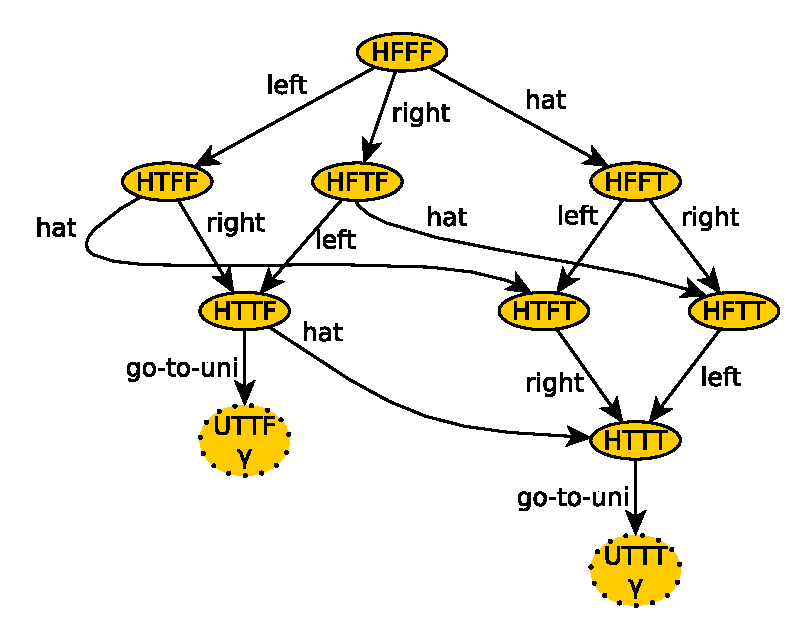
\includegraphics[scale=0.7]{breadthFirstBasic}
\caption{breadth-first search graph (with dublicate detection)}
\end{figure}

\subsection*{(b) Not finished yet.}
\subsubsection*{First Node Expansion}
Initial disjunctive action landmark: $L = \{\text{wear-left-shoe, wear-right-shoe}\}$ (ToDo: explain why)

Compute $T_S$:
\begin{enumerate}
\item Include wear-left-shoe in $T_S$ as disjunctive action landmark
\item no other applicable operators interfere with wear-left-shoe
\item for go-to-university, which is not applicable yet $T_S$ contains a necessary enabling set.
\end{enumerate}
$T_S = \{\text{wear-left-shoe}\}$

\subsubsection*{Second Node Expansion}
disjunctive action landmark: $L = \{\text{wear-right-shoe}\}$
Compute $T_S$:
\begin{enumerate}
\item Include wear-right-shoe in $T_S$ as disjunctive action landmark
\item no other applicable operators interfere with wear-right-shoe
\item for go-to-university, which is not applicable yet $T_S$ contains a necessary enabling set.
\end{enumerate}
$T_S = \{\text{wear-right-shoe}\}$

\subsubsection*{Third Node Expansion}
disjunctive action landmark: $L = \{\text{go-to-university}\}$
Compute $T_S$:
\begin{enumerate}
\item Include go-to-university in $T_S$ as disjunctive action landmark
\item Include hat in $T_S$ since it interferes with go-to-university (go-to-university disables hat)
\end{enumerate}
$T_S = \{\text{go-to-university, hat}\}$

\begin{figure}[h!]
\centering
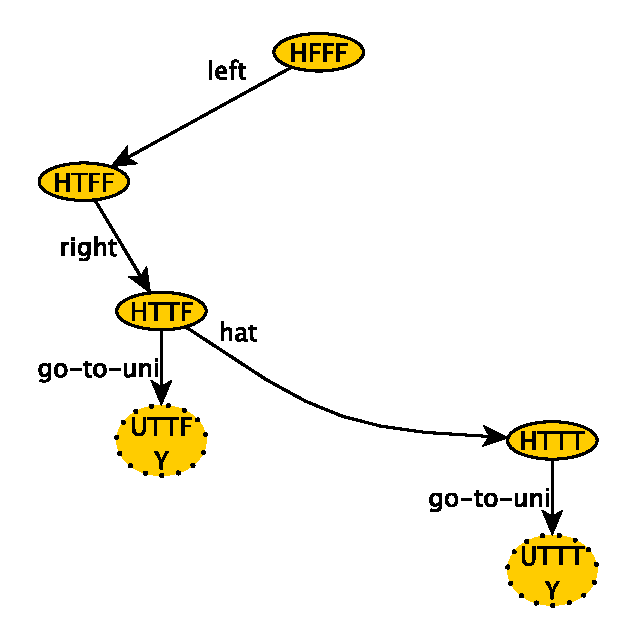
\includegraphics[scale=0.7]{breadthFirstStrongStubborn}
\caption{breadth-first search graph using strong stubborn set pruning}
\end{figure}

\subsection*{Conclusion}
11 vs 5 Node Expansions

\section*{Exercise 11.2}

\subsection*{Preliminaries}
For every variable $ v \in prevars(o) $ (Only for $o \in app(s)$?) we need to compute the Domain transition graph:
\begin{figure}[h!]
\centering
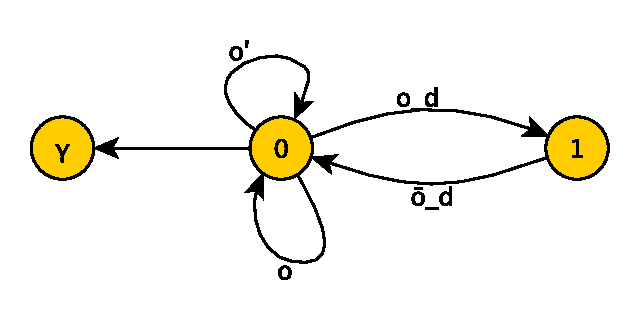
\includegraphics[scale=0.5]{DTG_a}
\caption{DTG(a)}
\end{figure}

All given operators are "Active Operators" (see lecture 13, slide 14), because of
\begin{itemize}
\item For every variable $v \in prevars(o)$ there is a path in $DTG(v)$ from $s(v)$ to $pre(o)(v)$.
\item If $v$ is goal-related, then there is also a path from $pre(o)(v)$ to the goal value $\gamma(v)$.
\end{itemize}

\subsection*{Disjunctive Action Landmark:}
$ L=\{o, o'\} $ in initial state

\subsection*{Strong Stubborn Sets}
\begin{enumerate}
\item Include $o$ (or $o'$) in $T_S$ as disjunctive action landmark.
\item Include $o_d$ in $T_S$ since it interferes with $o$ ($o_d$ disables $o$)
\item Include $o'$ (or $o$) in $T_S$ since it interferes with $o_d$ ($o_d$ disables $o'$)
\item Include $\overline{o_d}$ and $o_i$ in $T_S$ since both conflict with $o_d$
\item Include $\overline{o_i}$ in $T_S$ since it conflicts with $o_i$
\end{enumerate}
$T_S = \{o, o', o_d, \overline{o_d}, o_i, \overline{o_i}\} $

All six operators included in $T_S$, no pruning.

\begin{figure}[h!]
\centering
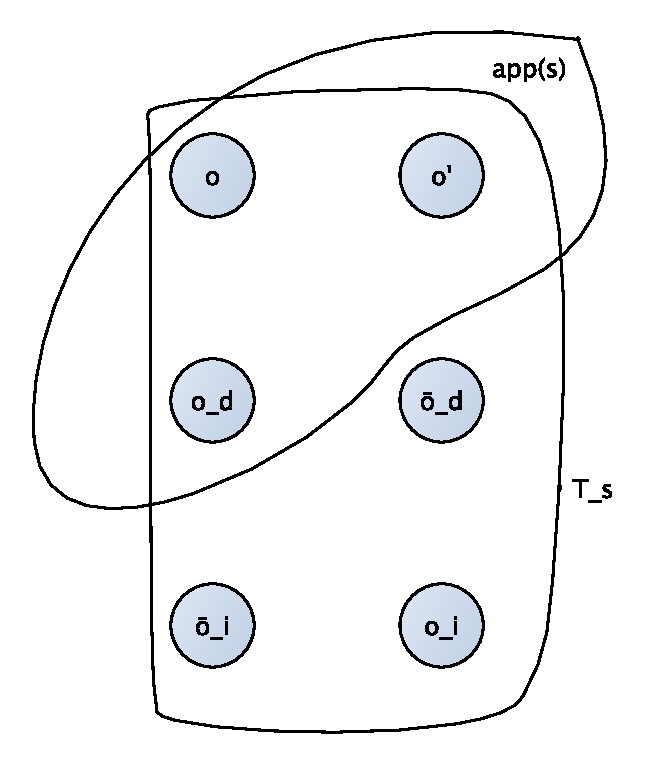
\includegraphics[scale=0.4]{strongStubborn}
\caption{strongStubborn}
\end{figure}

\subsection*{Weak Stubborn Sets}
\begin{enumerate}
\item Include $o$ (or $o'$) in $T_S$ as disjunctive action landmark.
\item there are no operators in $s$ that have conflicting effects with $o$ or that are disabled by$o$
\end{enumerate}
$T_S = \{o\} $

Nice amount of pruning.

\begin{figure}[h!]
\centering
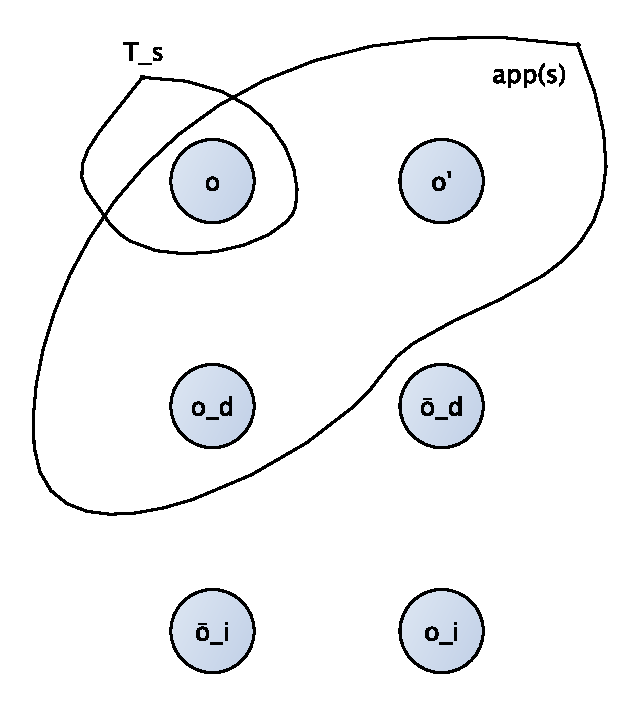
\includegraphics[scale=0.4]{weakStubborn}
\caption{weakStubborn}
\end{figure}

\subsection*{Conclusion}
Weak stubborn sets admit exponentially more pruning than strong stubborn sets.

\label{lastpage}
\end{document}
